\chapter{Cuadricoptero con vision artificial}\label{sec: Cuadricoptero}
En el presente capítulo se pretende abordar el diseño y la implementación de un cuadricóptero con la capacidad para el seguimiento de un objeto, haciendo uso para ello de una FPGA como parte fundamental, y algunas otras herramientas que se expondrán a lo largo de esta sección. \newline

\section{Diseño}
En la figura se presenta un esquema con un alto nivel de abstracción en el que se da una primera aproximación del funcionamiento del sistema general.

\begin{figure}[H]
	\center
	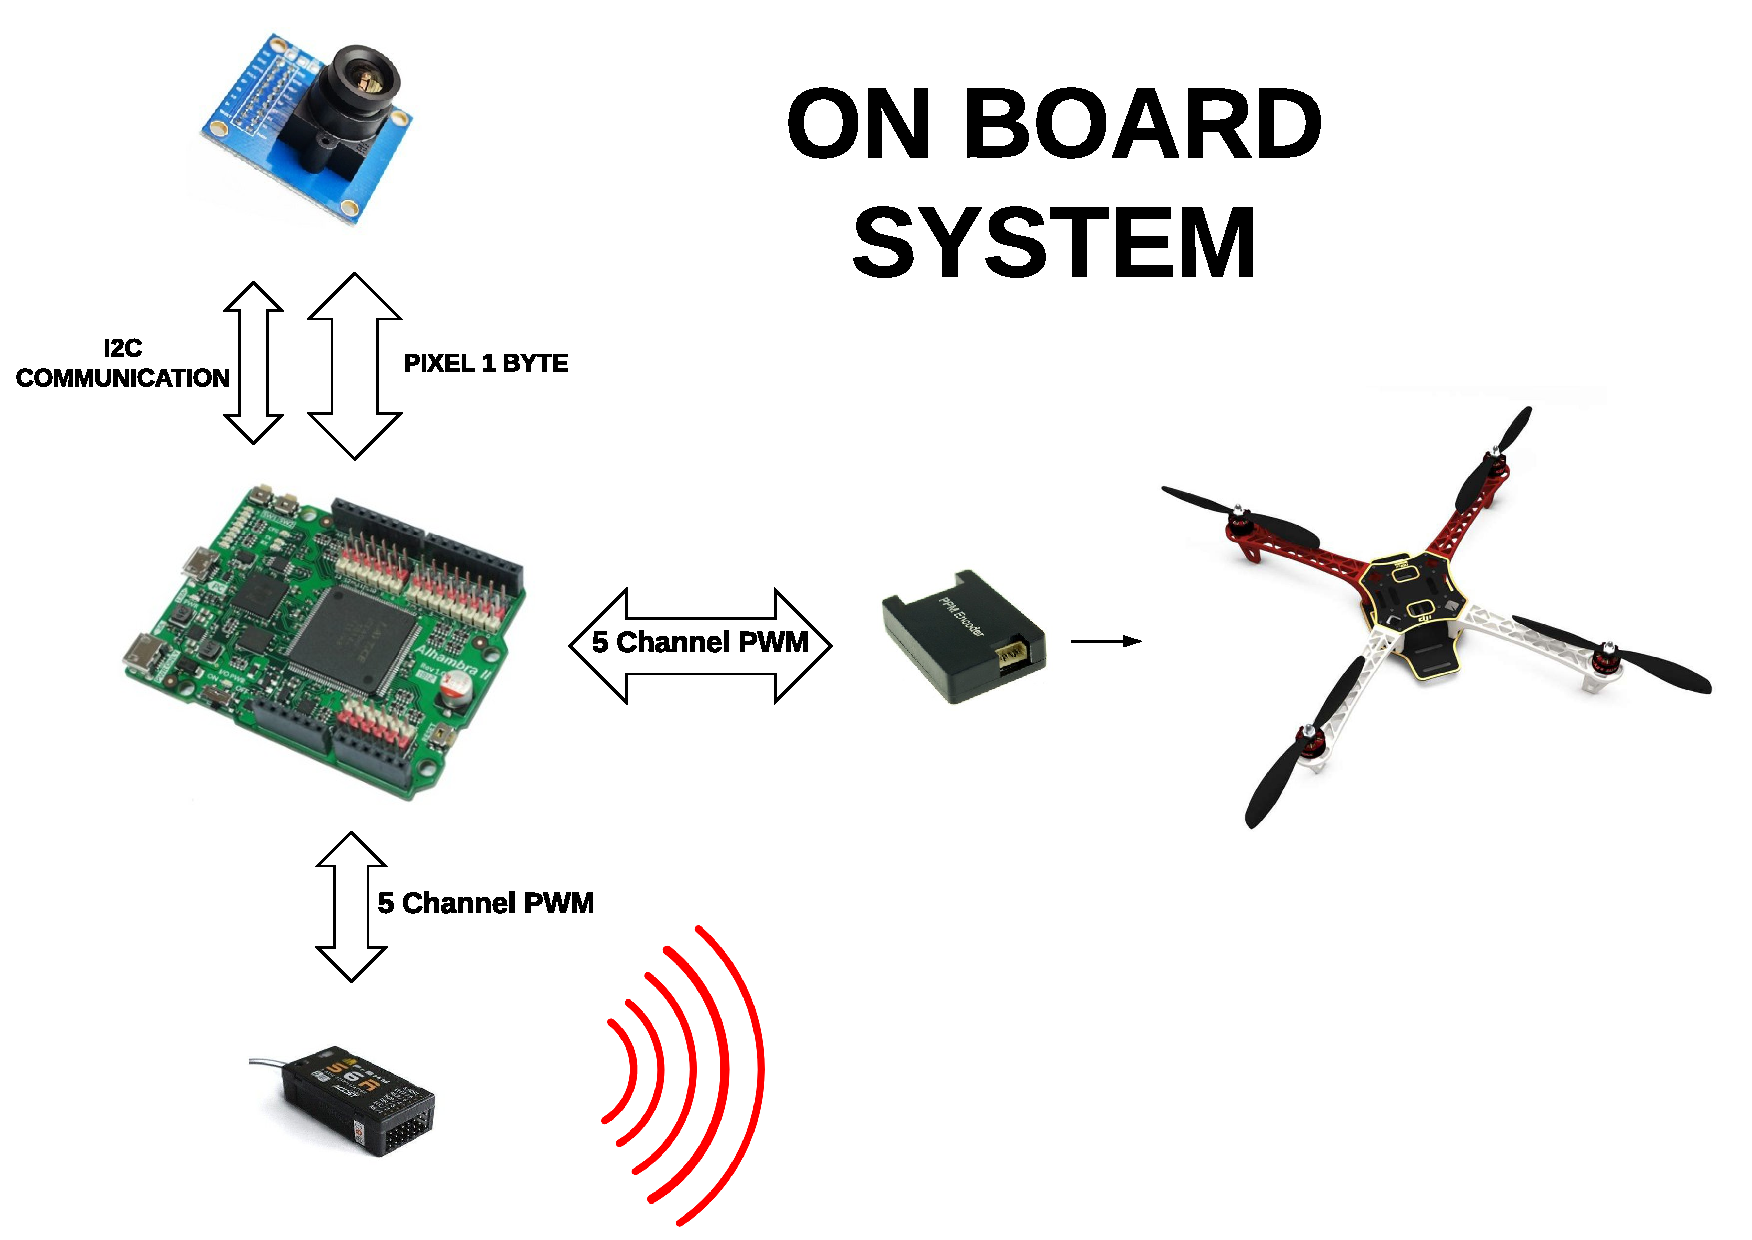
\includegraphics[trim = 0mm 4cm 0mm 4cm, clip,scale=0.5]{imagenes/Cuadricoptero_vision/on_board.pdf}
	\caption{Diseño a alto nivel del cuadricóptero con visión.}
	\label{fig:on_board}
\end{figure}


\section{Implementación de la percepción}
OV7670

I2C

\begin{figure}[H]
	\center
	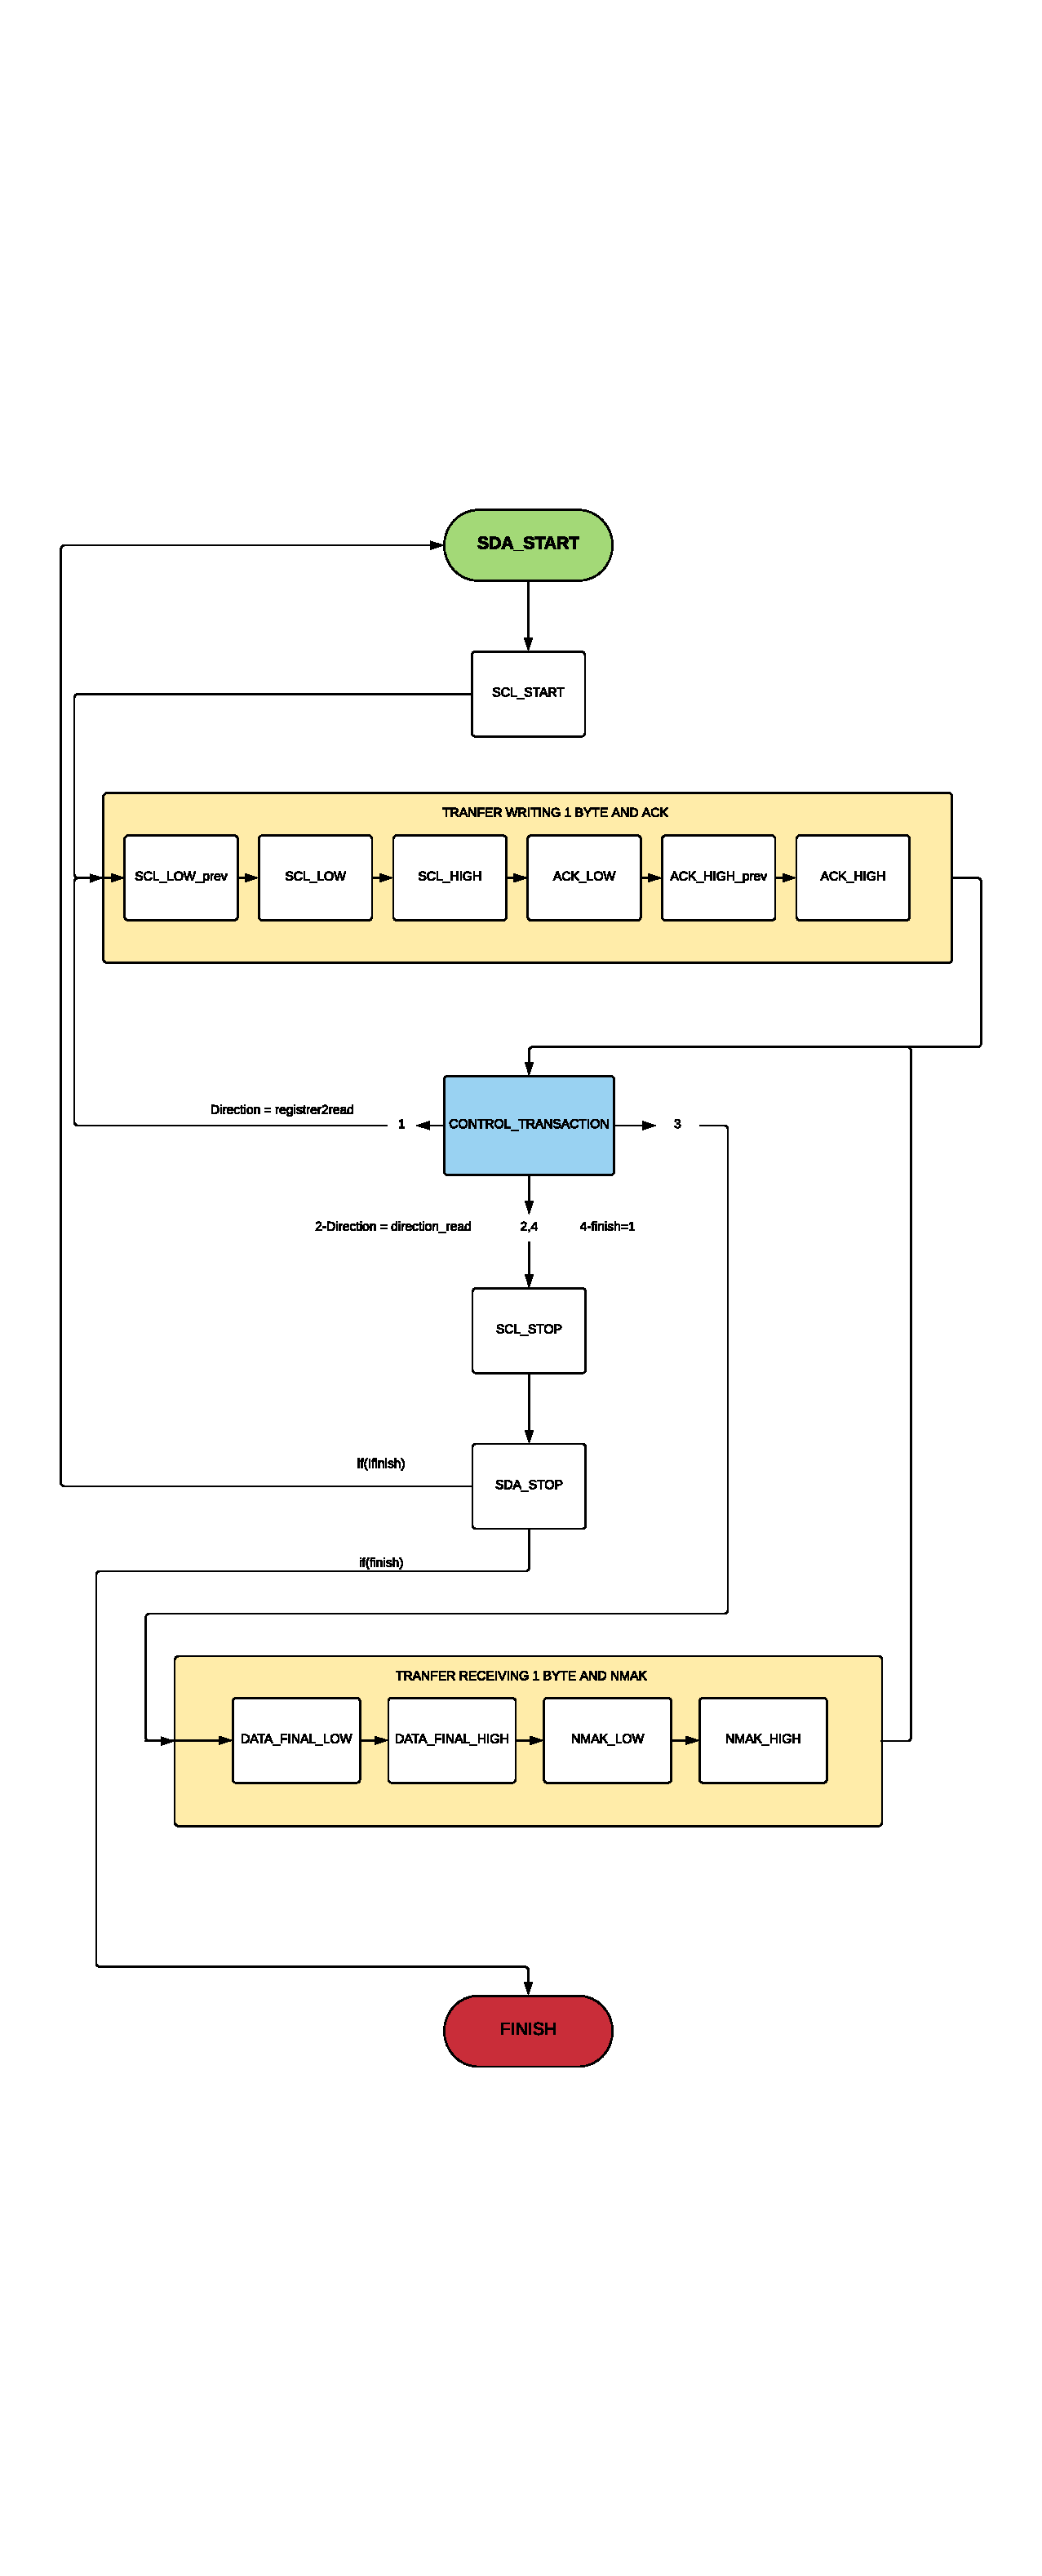
\includegraphics[trim = 0mm 0mm 0mm 0mm, clip,scale=0.5]{imagenes/Cuadricoptero_vision/I2C_WRITE.pdf}
	\caption{Diagrama de flujo de la escritura I2C.}
	\label{fig:i2c_write}
\end{figure}


Buscador de objeto


\section{Implementación del control}
\section{Experimentos}









